\section{Reordering}
Another method to decrease memory needed to solve the transport of
electron reorders the energy groups. When CEPXS creates the cross sections,
it first puts in all the cross sections for one particle and then the cross
section for the other particle into the scattering matrix. The cross section 
matrix looks like :
\begin{equation}
S = 
\begin{pmatrix}
A & B\\
C & D
\end{pmatrix}
\end{equation}
where $A$ and $B$ are lower triangular matrices which represents the
scattering for each particle. For each particle, only down scattering
is allowed because the cut-off energy forbids the thermalization of 
particles. The matrices $B$ and $C$ represent the creation of electrons by
photons through photo-electric effect and the creation of photons by
electrons through bremsstrahlung. Now it is important to notice that a
particle can only create a particle which has a energy lower than its own
energy. Moreover, CEPXS forces the maximum energy and the cut-off energy to
be the same for the two particles. For example, theres are two groups for the
photons and four groups for the electrons. The transfer between the groups will 
look \hbox{like :}
\begin{figure}[H]
\begin{center}
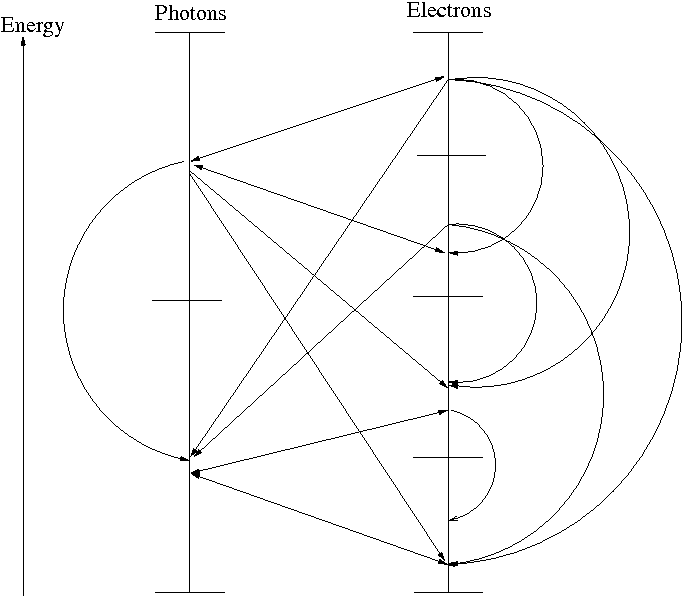
\includegraphics[height=7cm]{group.png}
\caption{Transfer between the different groups}
\end{center}
\end{figure}
The pattern of the scattering matrix looks like :
\begin{equation}
S =
\begin{pmatrix}
x & 0 & x & x & 0 & 0\\
x & x & x & x & x & x\\
x & 0 & x & 0 & 0 & 0\\
x & 0 & x & x & 0 & 0\\
x & x & x & x & x & 0\\
x & x & x & x & x & x\\
\end{pmatrix}
\end{equation}
We can see that there is no upscattering to the first group of photons, the
first and the second group of electrons coming from the second group of
photons and the third or the fourth group of electrons. Thus, if we reorder the 
groups using the following order : photon group 1, electron group 1, electron 
group 2, photon group 2, electron group 3, electron group 4. The pattern of the 
scattering matrix will look like :
\begin{equation}
S =
\begin{pmatrix}
x & x & x & 0 & 0 & 0\\
x & x & 0 & 0 & 0 & 0\\
x & x & x & 0 & 0 & 0\\
x & x & x & x & x & x\\
x & x & x & x & x & 0\\
x & x & x & x & x & x\\
\end{pmatrix}
\end{equation}
Now, we see that we can solve our problem by solving two problems with only three
groups each. We say that we have two group sets of three groups each. We can solve 
the first three groups without solving of the last three groups since there is no 
upscattering coming from these. Then, we can solve the last three groups, with 
the first three groups hidden in the source term. Thus, we can solve a problem
with six groups using the same memory that we would use for only three groups. To 
know how many groups we need to gather from each particle in each group set, we 
can use a simple rule. First, we define the number of groups of photons as
$n_p$, the number of groups electrons as $n_e$ and the greatest common divisor
between these two numbers as $gcd$. The number of groups of photons to put in
a group set is $\frac{n_p}{gcd}$ and the number of groups of electrons to put
in a group set is $\frac{n_e}{gcd}$. Instead of solving one problem of $n$ 
groups, we can solve $gcd$ problems of $\frac{n}{gcd}$ groups.


